\section{Orbit Altitude}
\label{mtrOrbAltitude}
During the design of the orbit, very careful attention has to be given to the choice of the mission altitude for the entire formation. This parameter is vital for the lifetime requirement.

Initially it was apparent that the choice of the emitting payload would give a hard altitude constraint, however as described in section \ref{mtDOLSR}, with the use of complex optical instruments it was possible to open a wider range of altitudes for selection. The governing properties of the orbit for altitude selection have now become the orbit perturbations.

This section details the considerations in regards to these properties. A separate radiation exposure analysis is also done. Finally a suitable altitude is chosen based on this analysis.
\subsection{Earth Oblateness}
\label{mtrOrbJ2}
The perturbation sensed by the satellite due to Earth's oblateness effect only influences the rate of precession of the orbit which is given in the following equation:

\begin{equation}
\dot{\Omega _{J_2}} = -1.5nJ_2 ( R_E / a )^2 ( cos i ) ( 1-e^2 )^{-2}
\label{j2eq}
\end{equation}

The rate of precession is a function of the semi-major axis, however $\dot{\Omega _{J_2}}$ does not affect altitude directly.

\subsection{Perturbations due to Other Celestial Bodies}
\label{mtrOrbSelestialBodies}
The gravitational forced of other celestial bodies like the Sun and the moon  cause periodic variations in all orbital elements, however in \ac{LEO} these perturbations are very minor (and above all are constant for formations) relative to atmospheric drag, thus will not be considered in this report.
\subsection{Solar Radiation Pressure}
\label{mtrOrbSolRadiation}
All orbiting bodies are affected by solar radiation pressure. The acceleration due to this phenomenon can potentially affect stationkeeping of the swarm if all satellites have different cross-sectional areas normal to the sun. This perturbation is not directly related to orbit altitude, however it is an important step in orbit analysis. In figure \ref{fig:solarRadArea} on page \pageref{fig:solarRadArea}, the relationship between the acceleration and the normal area to the sun for different satellite masses is shown. Similarly, a graph relating the mass to the acceleration for different cross-sectional areas is shown in figure \ref{fig:solarRadMass} on page \pageref{fig:solarRadMass}.

\begin{figure}[ht!]
\centering
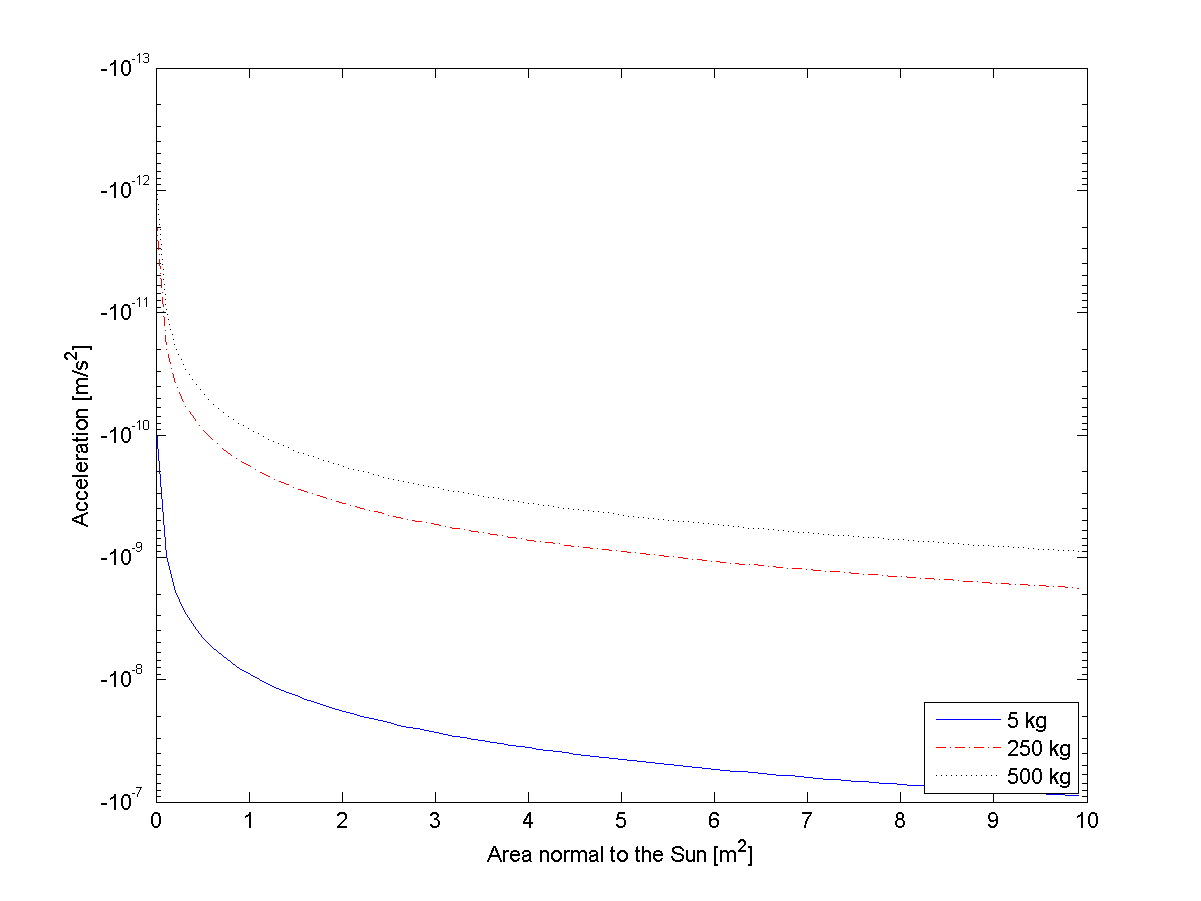
\includegraphics[width=0.8\textwidth, angle=0]{chapters/img/solPressureVarArea.png}
\caption{Acceleration due to solar radiation pressure vs. area normal to the sun, for different satellite masses.}
\label{fig:solarRadArea}
\end{figure}

\begin{figure}[ht!]
\centering
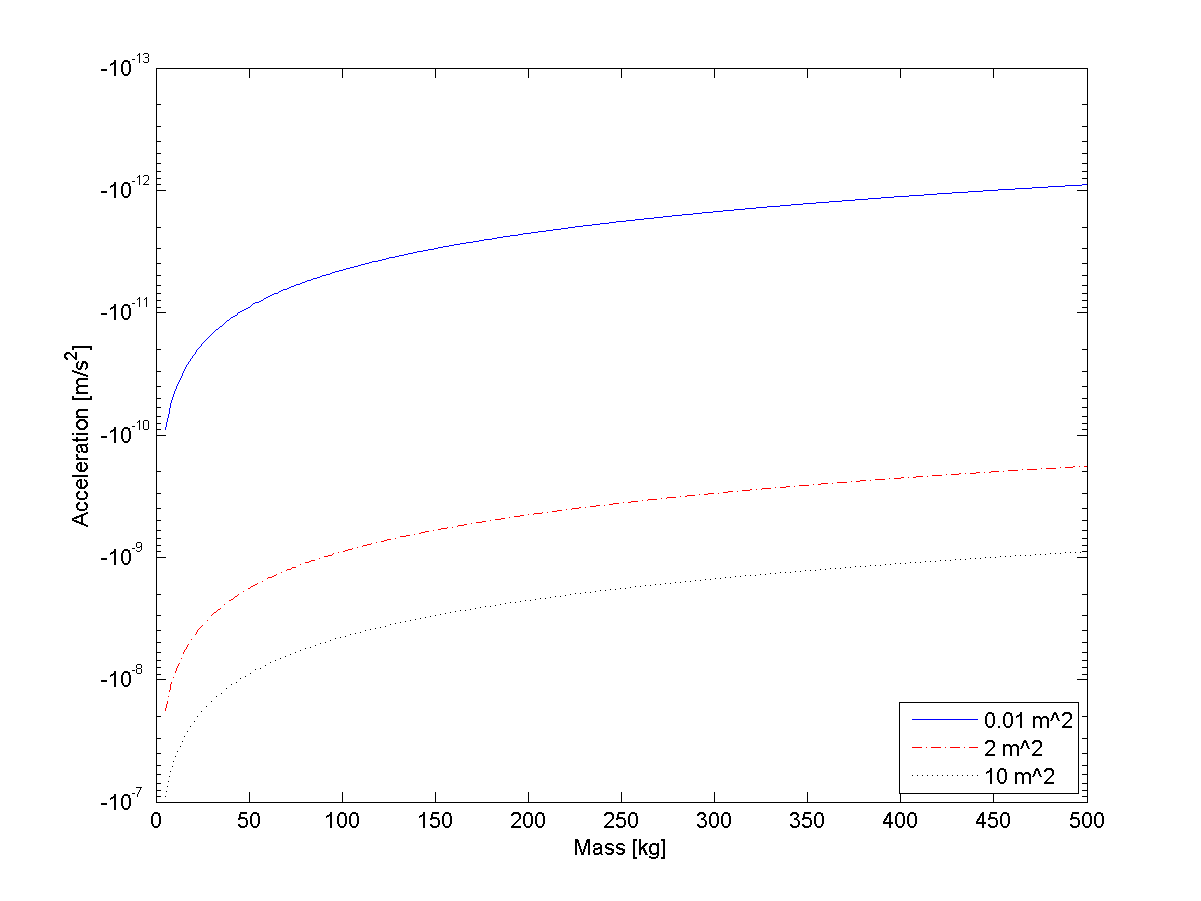
\includegraphics[width=0.8\textwidth, angle=0]{chapters/img/solPressureVarMass.png}
\caption{Acceleration due to solar radiation pressure vs. mass, for different areas.}
\label{fig:solarRadMass}
\end{figure}

These figures present design boundary overviews and a general feeling of behavior due to solar radiation pressure is shown. The inverse relationship is obvious. In order to minimize this perturbation it is required to have high mass while retaining the smallest possible area normal to the sun.

What is important to note is that if the ration of area to mass could be maintained constant between the emitting and the receiving satellites, then they would experience the same perturbation, which is a favorable condition. Acceleration with respect to this area/mass ratio can be seen in figure \ref{fig:solarRadRatio} on page \pageref{fig:solarRadRatio}.

\begin{figure}[h!]
\centering
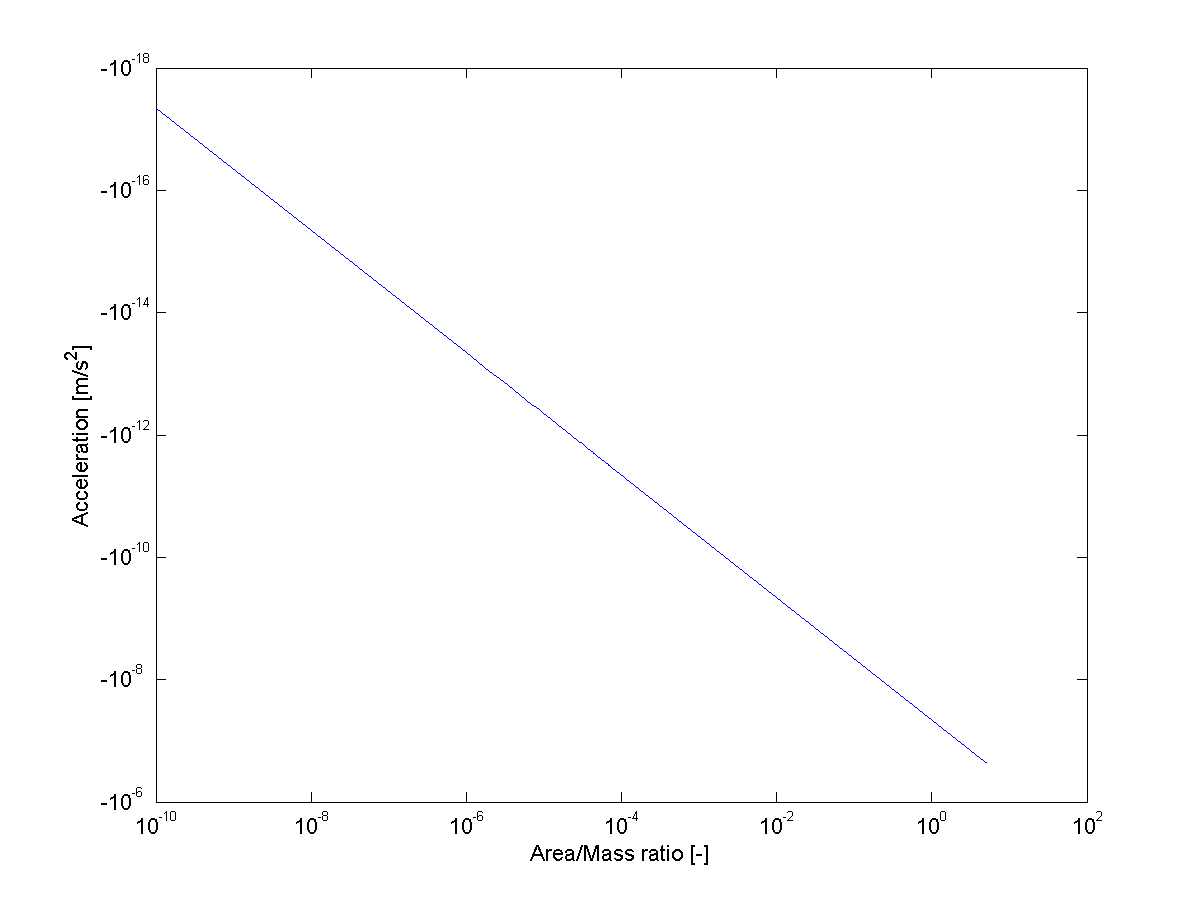
\includegraphics[width=0.8\textwidth, angle=0]{chapters/img/solPressureVarRatio.png}
\caption{Acceleration due to solar radiation pressure vs. Area/Mass ratio.}
\label{fig:solarRadRatio}
\end{figure}

\begin{table*}[h]
	\centering
		\begin{tabular}{c|c|c}
		 & Total Mass & Max. Area \\ \hline \hline
		 Emitter & 119 & 2.5 \\ 
		 Receiver & 10.7 & 0.2 
			
		\end{tabular}
	\caption{Mass and area estimates}
	\label{table:solarEstimates}
\end{table*}

Based on preliminary mass and area estimates shown in table \ref{table:solarEstimates} on page \pageref{table:solarEstimates}, it is estimated that the both the emitter and the receiver platforms will experience a decceleration in the order between 10\textsuperscript{-9} and 10\textsuperscript{-10}. While these values might not seem significant at first, especially relative to atmospheric drag (see section \ref{mtrAtmDrag}), they will become relevant for stationkeeping as explained earlier.

\subsection{Atmospheric Drag}
\label{mtrAtmDrag}

Atmospheric drag is by far the most relevant perturbation for \ac{LEO} satellites. It directly relates to mass as it influences the amount of fuel required to maintain the orbit, where as the mass influences the rate at which the orbit decays. Altitude selection relies heavily on estimation and analysis of drag data as for longer mission times, higher altitudes are preferred, while optical instruments prefer lower altitudes for increased accuracy.

The drag that the satellite experiences due to atmospheric density is described by the following formula:

\begin{equation}
D = -\frac{1}{2} C_D \rho V^2A
\label{drag}
\end{equation}

It follows that orbital parameter changes (semi-major axis, period and velocity respectively) per orbit are calculated using the following equations (assuming negligible eccentricity):

\begin{equation}
\Delta a = -2 \pi \left( C_D \frac{A}{m} \right) \rho a^2
\label{deltaSMA}
\end{equation}
\begin{equation}
\Delta P = -6 \pi \left( C_D \frac{A}{m} \right) \rho \frac{a^2}{V}
\label{deltaP}
\end{equation}
\begin{equation}
\Delta V = \pi \left( C_D \frac{A}{m} \right) \rho aV
\label{deltaV}
\end{equation}

The fundamental problem with accurately predicting effects due to atmospheric drag is twofold: firstly it is very hard to predict the satellite's ballistic coefficient:

\begin{equation}
\frac{m}{AC_D}
\label{ball}
\end{equation}

Even with a well known mass to area ratio, the coefficient of drag can be highly variable, highly dependent on the shape of the satellite and its orientation with respect to the velocity vector. Throughout the following analysis a $C_D$ of 4 has been used as a worst-case scenario. This value is representative of a flat plate traveling with its normal vector pointing in the direction of velocity. In reality this drag coefficient changes. The cross-sectional area normal to the velocity vector can also vary for the swarm satellites if the whole platform is reoriented for instrument pointing. The whole ballistic coefficient typically ranges from about 25 kgm\textsuperscript{-2} to 100 kgm\textsuperscript{-2}. The satellites being considered, at this early stage in the design process, have a much lower coefficient - in the range of 10 kgm\textsuperscript{-2}.

The second reason drag calculations are so unreliable, is because air density at any altitude is highly variable. Raising air density is primarily connected with solar activity. As solar activity increases every 11 years (see figure \ref{fig:solarCycle} for recorded and predicted solar activity), the atmosphere heats up. Contrary to conventional gas laws that would dictate a fall in density as the gas expands, the atmosphere simply rises, increasing density at higher altitudes.

\begin{figure}[ht!]
\centering
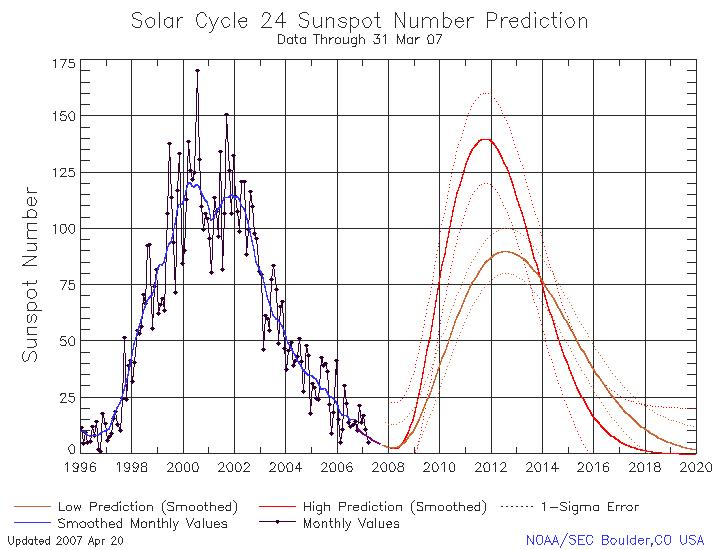
\includegraphics[width=0.9\textwidth, angle=0]{chapters/img/solarCycle.jpg}
\caption{The solar cycle, clearly showing the solar maxima at 11 year intervals. Data after 2007 is projected. \emph{Source: NASA} }
\label{fig:solarCycle}
\end{figure}

The density difference during maxima and minima for different altitudes is shown in figure \ref{fig:densityProfile}. Depending on the altitude, the density could vary for up to a whole order of magnitude between the minimum and maximum.

\begin{figure}[ht!]
\centering
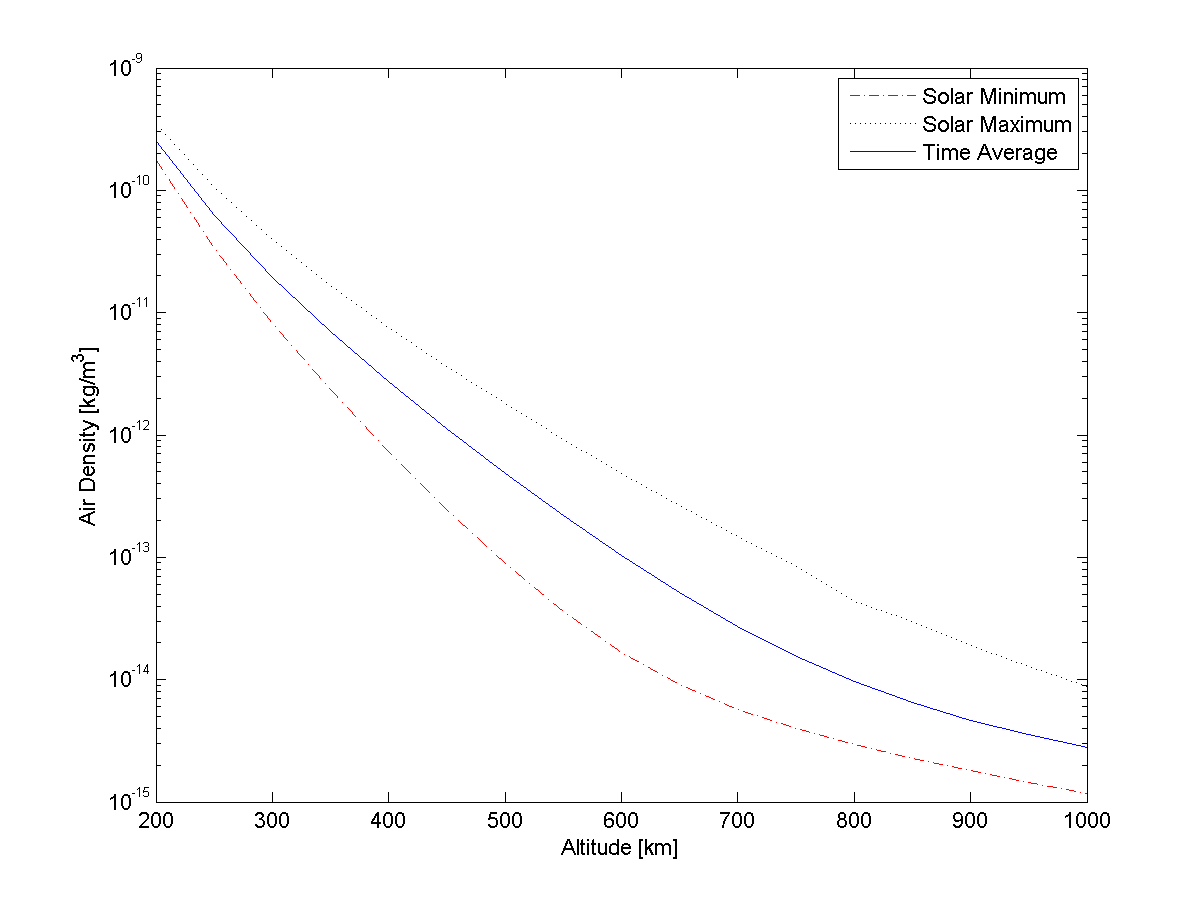
\includegraphics[width=0.9\textwidth, angle=0]{chapters/img/densityAltitude.png}
\caption{Air density vs. orbit altitude for different solar cycle stages.}
\label{fig:densityProfile}
\end{figure}

Orbit decay periods for the emitter and receiver satellites are shown in figures \ref{fig:decayEmitter} and \ref{fig:decayReceiver} respectively. The Orbit decay is calculated using equations \ref{deltaSMA} - \ref{deltaV}. Orbit maintenance is not taken into account. The time range considered is a 5 year mission lifetime. The basis for the receiving satellite sizing was taken to be around 0.2 m$^2$ (based on preliminary sizing) . The mass of the said satellite was the same as in table \ref{table:solarEstimates} on page \pageref{table:solarEstimates}. The emitter satellite is sized to be about 2.5 $m^2$ frontal area (including solar panels and communications arrays). The mass is again taken from table \ref{table:solarEstimates}.

\begin{figure}[h!]
\centering
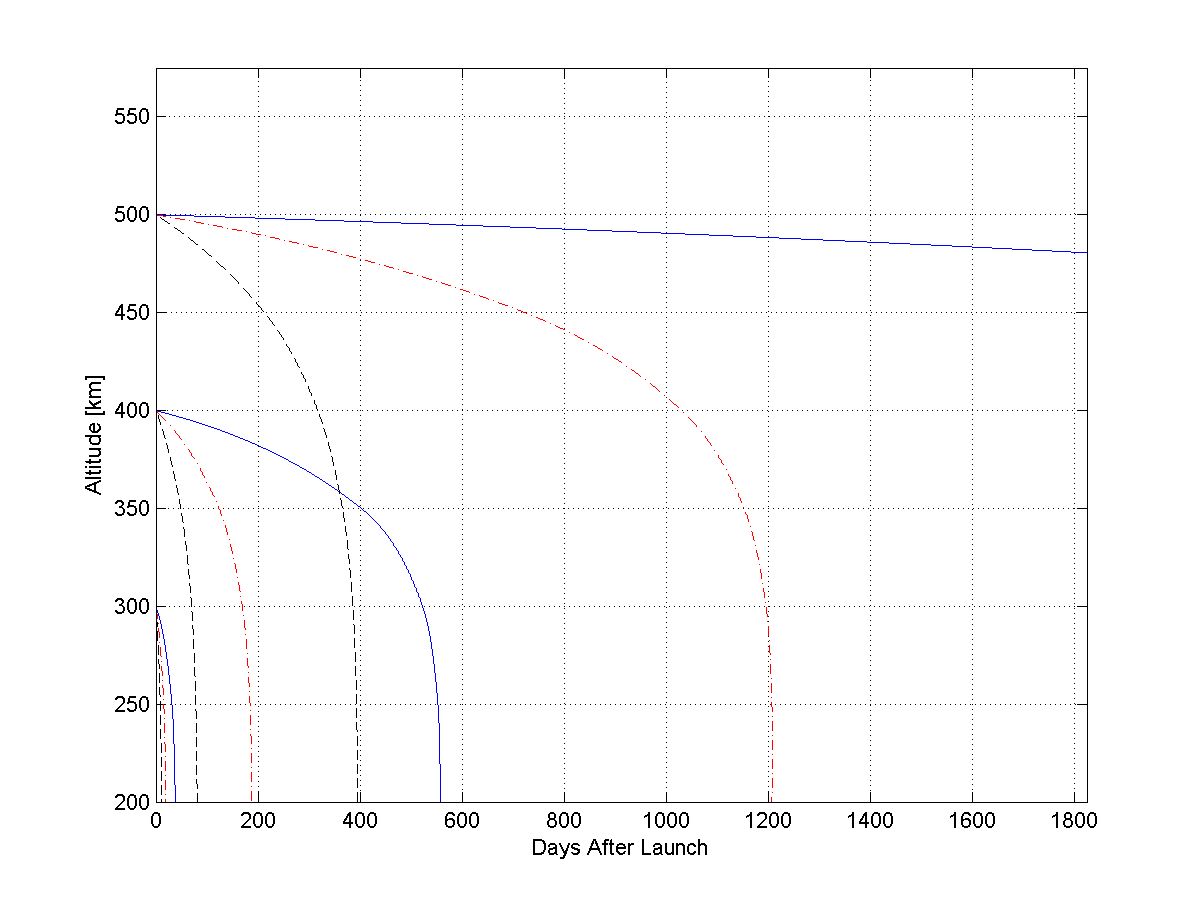
\includegraphics[width=0.95\textheight, angle=90]{chapters/img/orbitDecayEmitter.png}
\caption{Orbit decay for a satellite with $C_D$ = 4, A = 2.5 $m^2$ and m = 119 kg. Estimates for initial orbital altitudes of 300, 400 and 500 km at solar maximum (- -), solar minimum (--) and time average (-.-).}
\label{fig:decayEmitter}
\end{figure}

\begin{figure}[h!]
\centering
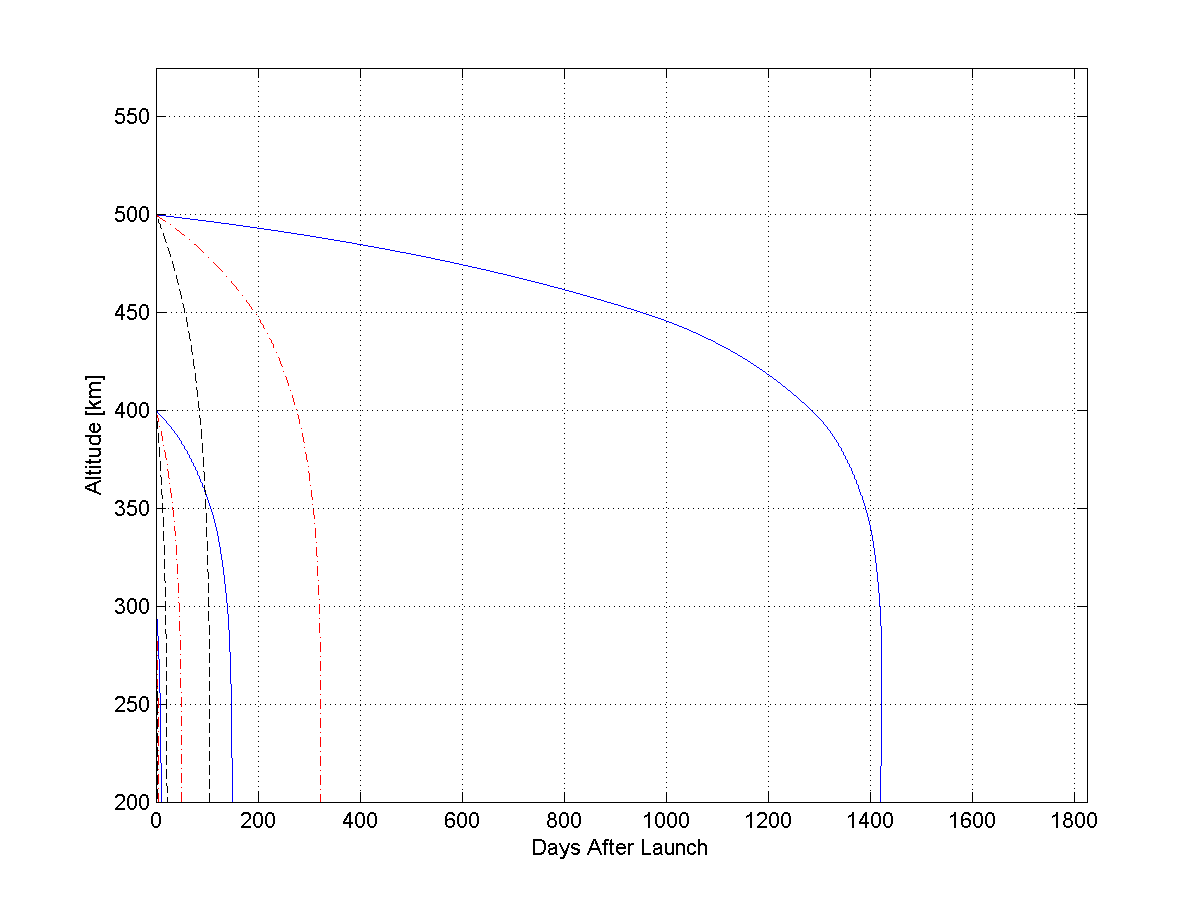
\includegraphics[width=0.95\textheight, angle=90]{chapters/img/orbitDecayRecieverMin.png}
\caption{Orbit decay for a satellite with $C_D$ = 4, A = 0.2 $m^2$ and m = 10.7 kg. Estimates for initial orbital altitudes of 300, 400 and 500 km at solar maximum (- -), solar minimum (--) and time average (-.-).}
\label{fig:decayReceiver}
\end{figure}

From the analysis of the orbit decay it is strikingly obvious how important the solar activity is during mission lifetime. Even at an altitude of 500 km neither satellite would be able to maintain its orbit for more then a 100 days. From this analysis it is clear that substantial orbit maintenance is required as the satellites will most probably not have refocusing equipment for the optical instruments. A more comprehensive idea of the orbit maintenance can be gathered from total $\Delta$V estimations shown in figures \ref{fig:deltaVGraph1} and \ref{fig:deltaVGraph2} (pages \pageref{fig:deltaVGraph1} and \pageref{fig:deltaVGraph2}) and tabulated in table \ref{table:deltaVTable} on page \pageref{table:deltaVTable}. This is the total velocity change required to keep the satellites in a certain circular orbit. The calculations are based on equation \ref{deltaV}.

